\documentclass{standalone}

\usepackage{tikz}
\usetikzlibrary{patterns,patterns.meta}

\begin{document}
    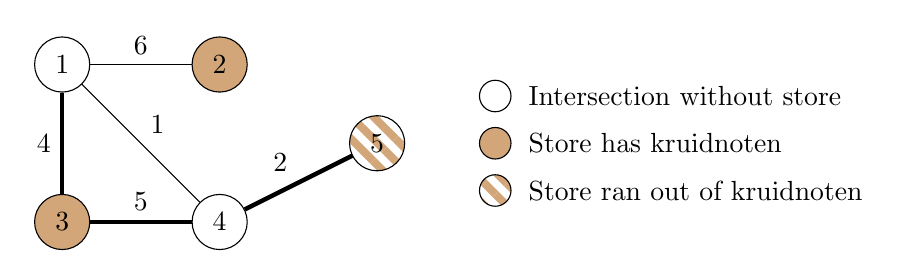
\begin{tikzpicture}[node/.style={draw, circle, minimum size=7mm}]
        \tikzstyle{hashed}=[pattern={Lines[angle=-45, distance=2mm, line width=1mm]}, pattern color=brown!70, outer sep=0pt]
        \node[node]                (1) at (0,  0) {$1$};
        \node[node, fill=brown!70] (2) at (2,  0) {$2$};
        \node[node, fill=brown!70] (3) at (0, -2) {$3$};
        \node[node]                (4) at (2, -2) {$4$};
        \node[node, hashed]        (5) at (4, -1) {$5$};

        \draw              (1) -- node[above]{$6$} (2);
        \draw[ultra thick] (1) -- node[left]{$4$} (3);
        \draw              (1) -- node[above right]{$1$} (4);
        \draw[ultra thick] (3) -- node[above]{$5$} (4);
        \draw[ultra thick] (4) -- node[above left]{$2$} (5);

        \node[node, minimum size=4mm]                at (5.5, -0.4) {};
        \node[node, minimum size=4mm, fill=brown!70] at (5.5, -1.0) {};
        \node[node, minimum size=4mm, hashed]        at (5.5, -1.6) {};
        \node[anchor=west] at (5.8, -0.4) {Intersection without store};
        \node[anchor=west] at (5.8, -1.0) {Store has kruidnoten};
        \node[anchor=west] at (5.8, -1.6) {Store ran out of kruidnoten};
    \end{tikzpicture}
\end{document}
